%Chapter 12


\chapter{Delta- A Moving Target}\label{ch:Delta- A Moving Target}

\begin{figure}[H]
  \centering
    
\includegraphics[width=0.7\textwidth]{Images/Ch12/chapter12pic1.png}
\end{figure}

\lettrine{B}{e}fore you take the delta ball and run with it, the big thing you need to understand is that delta changes with the wind, and as a retail investor you cannot use simple arithmetic to accurately extrapolate future option values from delta.

Although delta tells you the expected change in the value of an options premium given an underlying stock’s change in value, it never really predicts the dollar change in an option due to a move in the underlying security past a given instant. This is because delta is a moving target (a derivative of stock price describing an instantaneous value- the change in option price). 

\section{Delta Changes Constantly,\\ Whenever the Price of the\\ Underlying Security Changes}

When the delta changes, the options premium accelerates faster as the underlying price changes, typically resulting in a larger move than predicted if the price action happened with a fixed delta. Delta is itself a variable derived from, and dependent on, the changes it describes.\footnote{The derivative of delta that describes how fast delta changes is gamma, covered in the next chapter.}  

To illustrate, from our example with the stock sitting at \$9.81, and the delta of the \$14 call at 0.0378. You’d expect the price of the call to go up 3.78 cents per dollar move in the underlying- That’s our definition. Right??? 

Yes, but if the price of the stock raises \$5 to \$14.81, there’s no way the price of the \$14 strike call is only going to go up 15.12 cents! 

\begin{figure}[H]
  \centering
    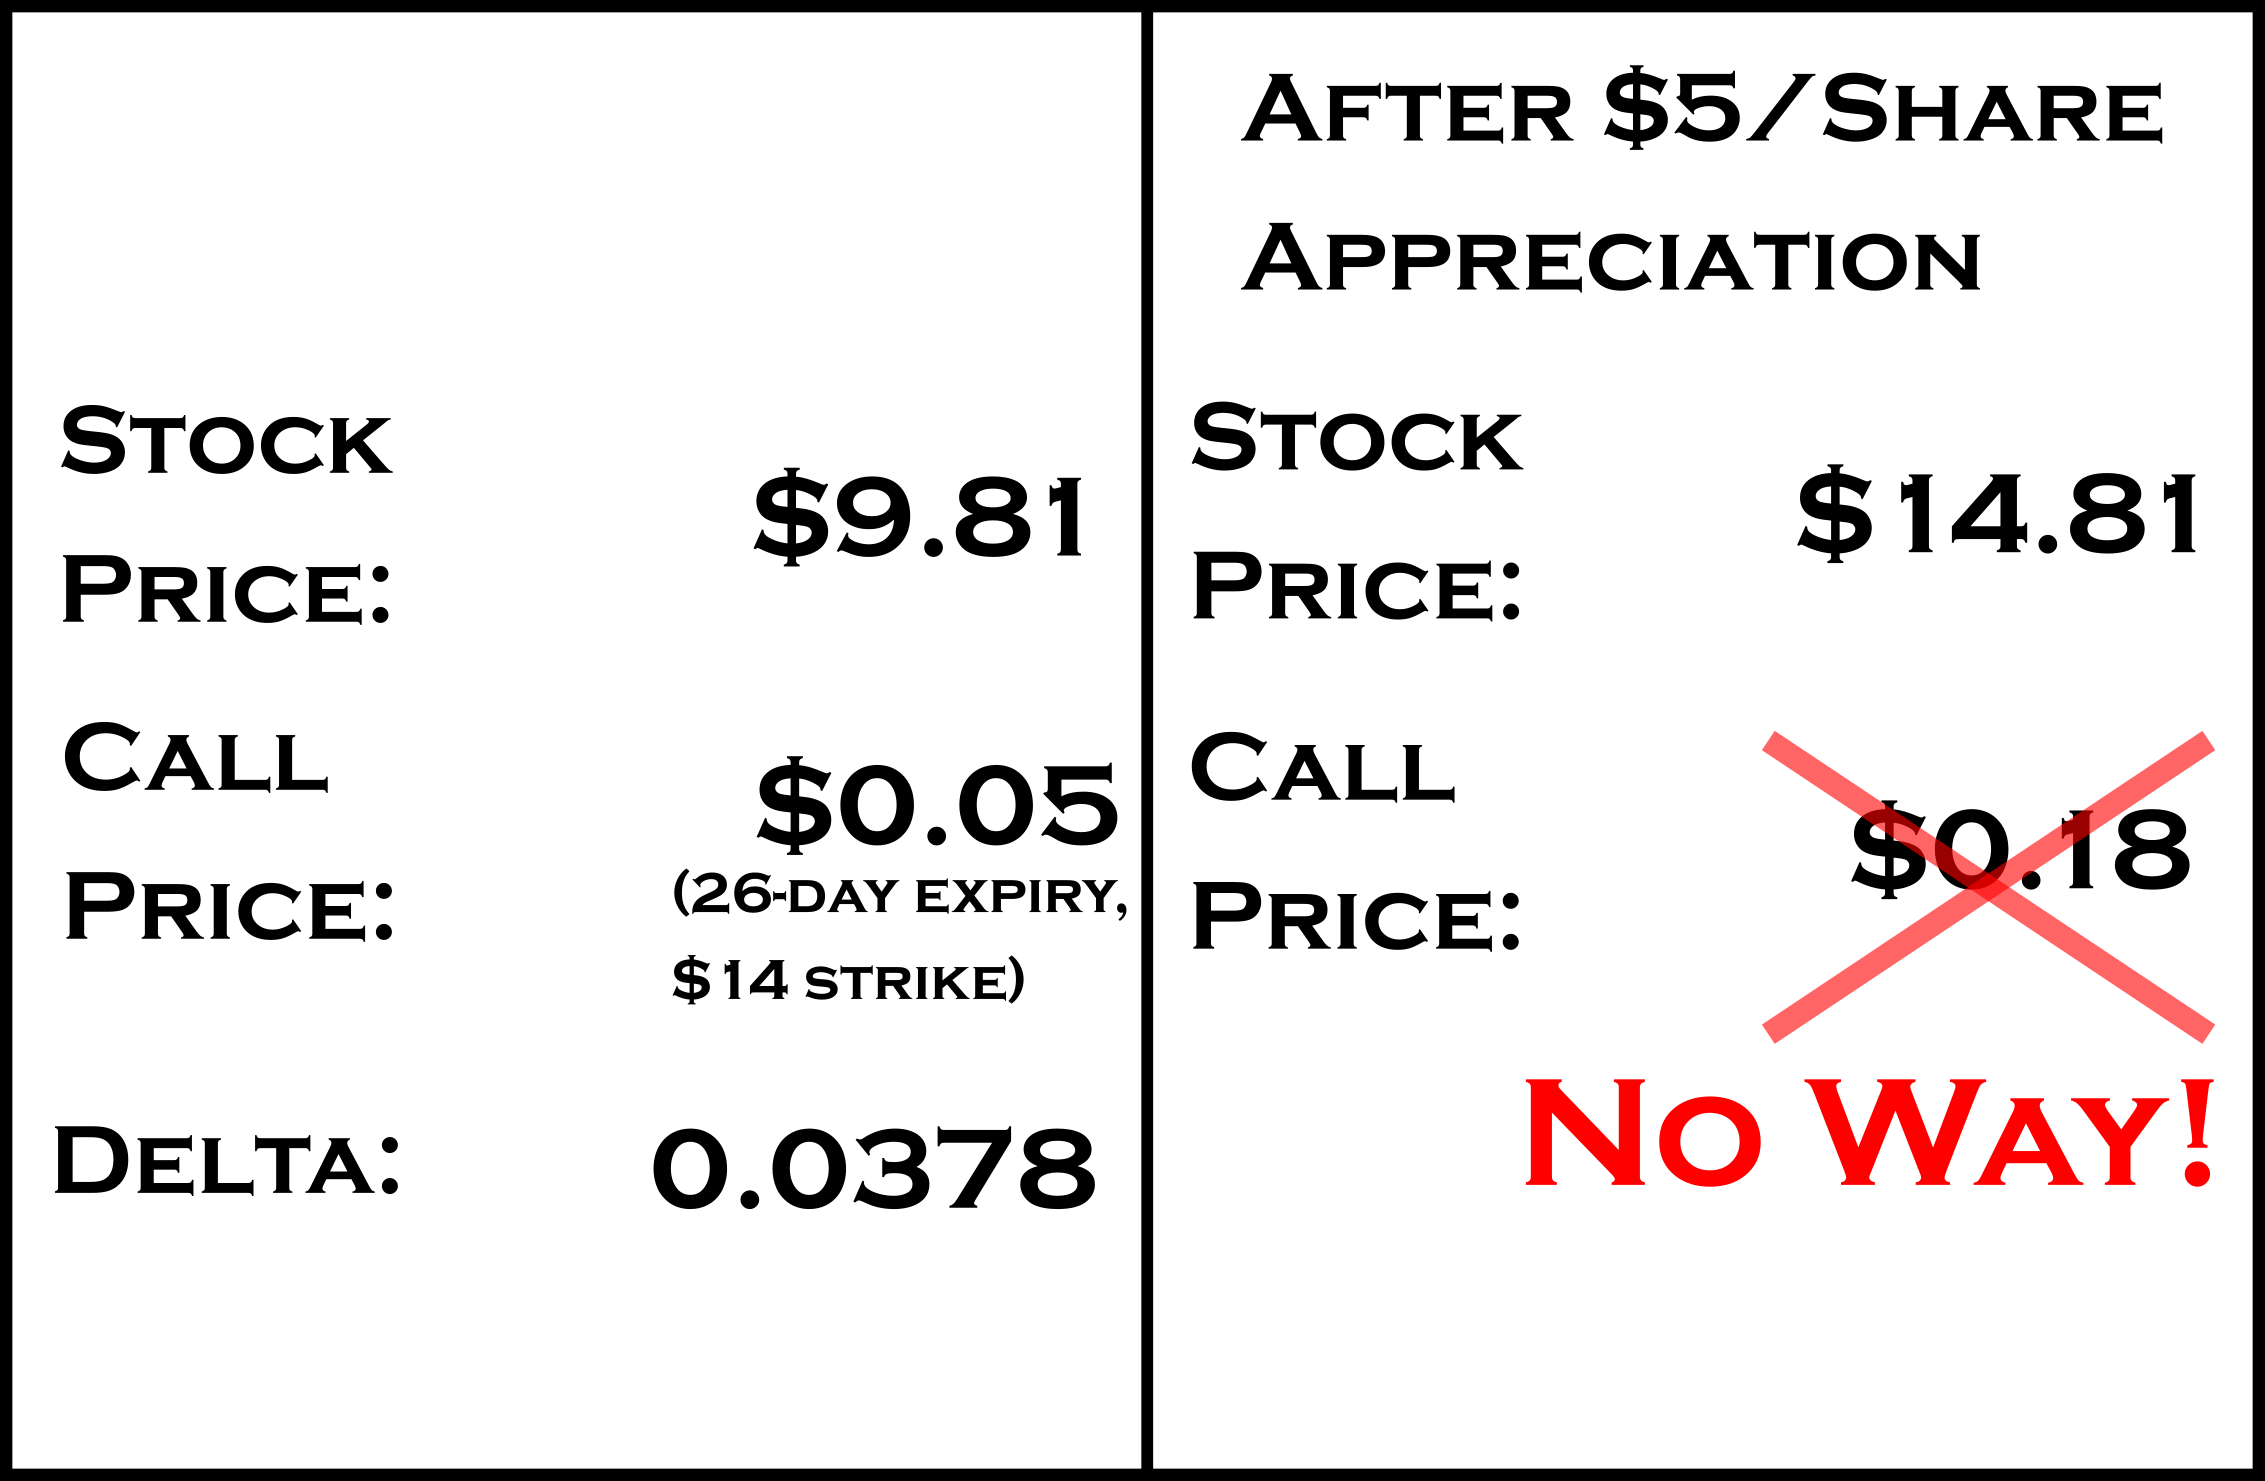
\includegraphics[width=0.9\textwidth]{Images/Ch12/chapter12pic2.png}
\end{figure}

That call is now in the money, it’s going to be worth way more than 18 cents. Just think about it- with the stock price at \$14.81, the \$14-strike call is worth 81 cents in intrinsic value alone! 

\section{As Delta Increases, the Option\\ Premium Increases Even Faster}

So what happened? As the price of the underlying changed, the value of the option and its delta also changed. When the underlying rose, it approached, and then became ITM (in the money). In turn, delta rose closer to 1, which describes the price of the option increasing faster and faster.\footnote{This is an example of what happens as you travel across the moneyness range and up the curve in the graph representing delta vs moneyness in the last chapter.} 

So what would the \$14 call with the stock at \$14.81 look like? I don’t have the mathematical model to spit out an exact number, but I can tell you that it is going to look way more like a call that is currently 81 cents in the money- the \$9 call. That call is going for \$1.45 [1.35-1.55 bid-ask]. With \$0.64 extrinsic value, you could ballpark with the stock at \$14 that the \$14-strike call would be going for \$1.45\footnote{Again, just for fun, notice \$0.03 to \$1.45 is a 2900\% return if you were the buyer of the call. This is how call buying can leverage small initial investments into massive returns. The hardest part is finding out what stock, and perhaps more importantly when, to YOLO.} or more (most likely more because the big move up would cause implied volatility, and in turn call value, to spike), and now have a similar delta.  It’s not a perfect estimate, but it is an estimate with enough utility to serve our needs.

\begin{figure}[H]
  \centering
    
\includegraphics[width=0.9\textwidth]{Images/Ch12/chapter12pic3.png}
\end{figure}

Knowing this should prepare you for what happens when the underlying changes and the value of your sold calls changes, and keep you from being disappointed by incorrect expectations based on the Delta “snapshot” in time you may have based your strategy on. With all this in mind, it's time to talk about our good friend, gamma.